\red{\begin{itemize}
    \item scrivere la differenza tra i FE
    \item fare disegno uguale a quello del mascheramento però con solo due coordinate
    \item scrivere delle misure cambiando i parametri del FE, e rifare le misure del FE con oscilloscopio e qualche plot
    \item scrivere misure del tempo morto e rifarle
\end{itemize}}

The TJ-Monopix1 is one of the chips fabricated by ToweJazz with 180 CMOS imaging process. From the middle of 2013 a dedicated collaboration, RD 53 ('Development of pixel readout integrated circuits for extreme rate and radiation'), has been established with the specific goal to find a sensor suitable as vertex detector for future upgrade of CMS and ATLAS experiments. Among the main objects of study of the collaboration there are both hybrid pixels and monolithic options as CMOS MAPS: fig \ref{fig:TJ180nm} shows the intermediate MAPS-prototypes made by TowerJazz.\\
\begin{figure}[h!]
    \centering
    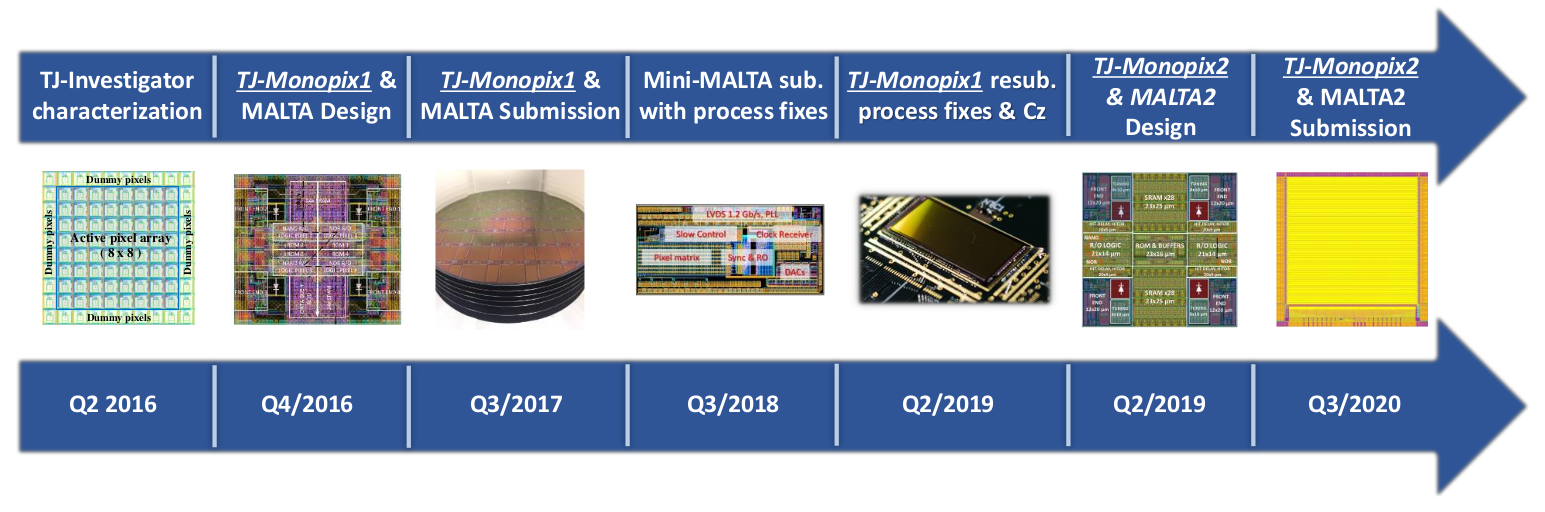
\includegraphics[width=.95\linewidth]{figures/Monopix1/TJ180nm.png}
    \caption{Timeline in TowerJazz productions.  In addition to Monopix series also the small electrode demonstrator TJ-Malta and mini-Malta have been produced and tested\cite{MALTA}. The Malta prototypes differ from TJ-Monopix in the readout: while Monopix implements a column-drain R/O, an asynchronous R/O without any distribution of BCID has been used by TJ-Malta in order to reduce power consumption.}
    \label{fig:TJ180nm}
\end{figure} 
Besides the TowerJazz series, also LFoundry fabricated other similar sensors with 150 CMOSS technology~\cite{LF-Monopix}\cite{LF-TJ-Monopix}: LF-Monopix.\\
The main differences between the LFoundry and TowerJazz's products (tab. \ref{tab:LF-TJ-Monopix}), are in the sensor structure rather than in the readout architecture, based on a column drain R/O with ToT capability (LF-Monopix has 8 bits dedicated and TJ-Monopix 6 bits). Concerning the sensor, LFoundry pixels are bigger and have a large-fill factor, while TJ-Monopix ones have a small fill-factor electrode.

The performances of both the detectors have been tested before and after irradiation ($\sim 10^{10} n_{eq}/cm^{2}$) and the result is, as expected since LF-Monopix is a large fill factor electrode (chap. \ref{chap:}), that LF-Monopix is more radiation hard than TJ-Monopix whereas the main degradation of efficiency in TJ-Monopix chips is due to the low electric field in the pixel corner. On the other hand one more accidental consequence of the large fill factor size in LF-Monopix (the deep p-well covers $\sim$ 55 $\%$ of the pixel area) is a significant cross-talk problem.
\begin{table}
    \begin{center}
    \begin{tabular}{|c | c |c |}
    \hline
    & LF-Monopix1 & TJ-Monopix1\\
    \hline
    \hline
    Bulk & p-type substrate & p-epi. on a low $\rho$ substrate \\
    Resistivity & $maggiore$ 2k$\Omega$cm & maggiore 1k$\Omega$cm\\
    Pixel size & 50 x 250 $\mu m^2$ & 26x40 $\mu m^2$ \\
    Depth & 100-750 $\mu$m & 25 $\mu$m \\
    Capacity & $\sim$ 400 fF & $\sim$ 3 fF\\
    Preamplifier & CSA & Voltage \\
    Threshold trimming & on pixel (4-bit DAC) & global threshold\\
    Readout mode & Fast column drain & Fast column drain\\
    Consumption & $\sim$ 300 mW/$cm^2$& $\sim$ 120 mW/$cm^2$ \\
    Threshold & 1500 $e^-$ & $\sim$ 270 $e^-$ \\
    ENC & 100 $e^-$ & $\sim$ 30 $e^-$\\
    \hline
    \end{tabular}
    \caption{Main characteristics of TJ-Monopix and LF-Monopix \cite{LF-TJ-Monopix}}
    \label{tab:LF-TJ-Monopix}
    \end{center}
 \end{table}

\section{The sensor}
    TJ-Monopix1 adopts the modification described in \ref{chap:a_modified_sensor} that allows to achieve a planar depletion region near the electrode applying a relatively small reverse bias voltage: a low dose n implant is build on a high resistivity ($\geq $ 1 k$\Omega$ cm), p-type epitaxial layer.\\
    This modification improves the efficiency of the detector, especially after irradiation\cite{}; however a Technology Computer Aided Design (TCAD) simulation has shown that a nonuniform electric field is still produced in the lateral regions after the modification; since the transversal component of the electric field drops at the pixel corner (this point in figure \ref{fig:Monopix1_section_scheme} is indicated by a star) the efficiency at the side is reduced. \\
    On a sample of chip, the one I've tested in Pisa belongs to these, a second optimization have been made to enhance the lateral component of electric field and improve the efficiency and velocity in charge collection near the corners of the sensor: a portion of low dose implant has been removed, creating a step discontinuity in the pixel corner. 
    A side effect is the weaker separation between the deep p-well and the p-substrate, that cannot be biased separately anymore to prevent the punchthrough. 
        \begin{figure}[h!]
        \centering
        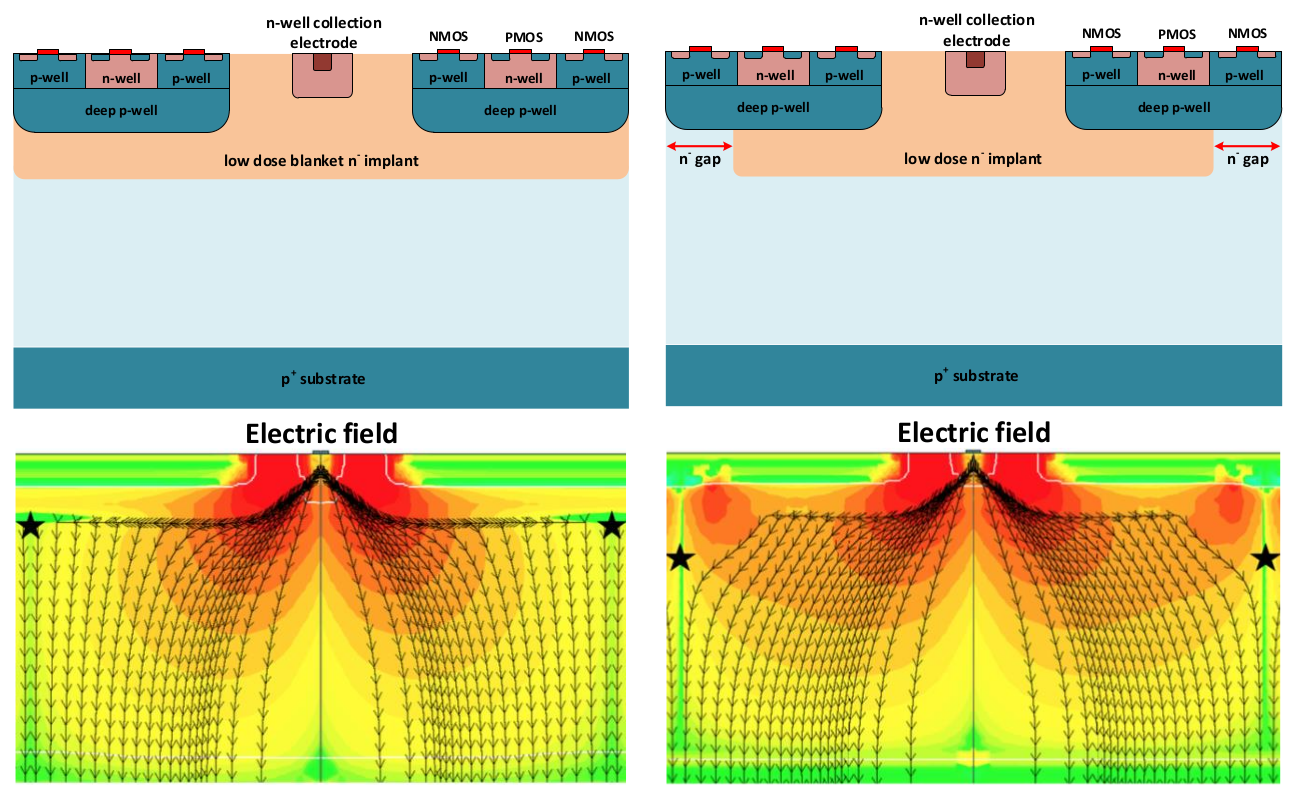
\includegraphics[width=.9\linewidth]{figures/Monopix1/Monopix1_section_scheme.png}
        \caption{(a) The cross-section of a monolithic pixel in the TJ-Monopix 180 nm with modified process; additionally in (b) a gap in the low dose implant is created to improve the collection of charge due to a bigger lateral component of the electric field}
        \label{fig:Monopix1_section_scheme}
    \end{figure}
    \begin{table}
        \begin{center}
        \begin{tabular}{| c |c |}
        \hline
        Parameter & Value\\
        \hline
        \hline
        Matrix size & \\
        Pixel size & 26x40 $\mu m^2$\\
        Depth & 25 $\mu$m \\
        BCID & 40 MHz \\
        ToT-bit & 6 \\
        Power consumption & $\sim$ 120 mW/$cm^2$\\
        \hline
        \end{tabular}
        \caption{}
        \label{tab:LF-TJ-Monopix}
        \end{center}
    \end{table}
    Moreover, to investigate the charge collection properties, as the threshold, the noise and the efficiency, pixels within the matrix feature a difference in the doping structure of the deep p-well: rows from 0 to 111 are fully covered by deep p-well (FDPW) under p-well near the sensor, while rows from 112 till the last 223 have a portion of deep p-well removed (RDPW). \\
    The removing enhance the lateral electric field component then resulting in a higher efficiency, as we'll see later.\\

\section{FE flavors}
    TJ-Monopix1 has been implemented in four different flavors, each one corresponding to a different sector on the matrix (fig. \ref{fig:Monopix1_flavors}) and thus having a separate readout and data transmission, in order to explore different variations of the FE. The four flavors mainly differ in the reset input circuit.
    \begin{figure}[h!]
        \centering
        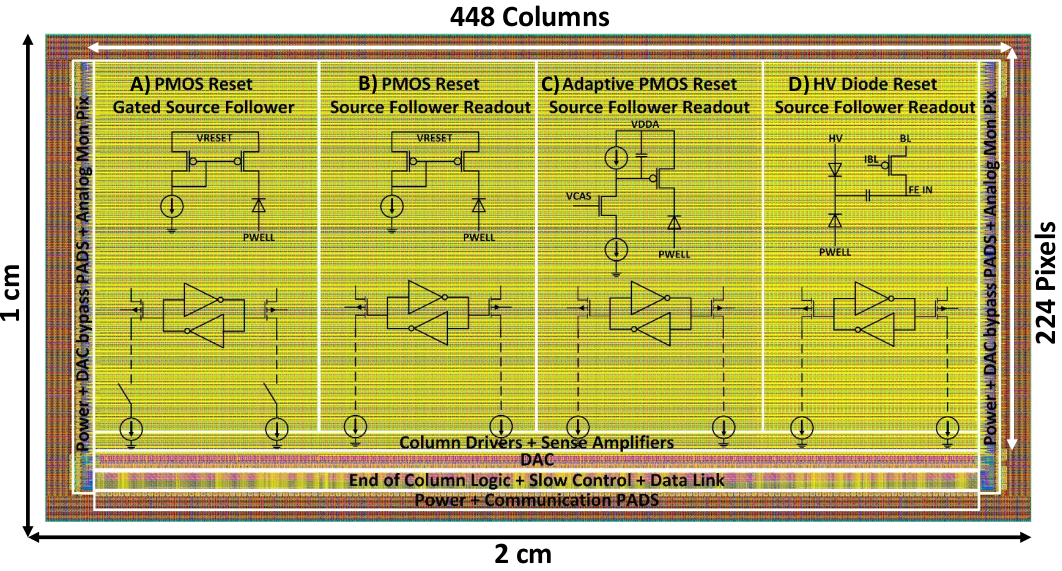
\includegraphics[width=.5\linewidth]{figures/Monopix1/Monopix1_flavors.png}
        \caption{}
        \label{fig:Monopix1_flavors}
    \end{figure}
    R resistenza di reset deve essere abbastanza grande in modo da far si che il ritorno allo zero è abbastanza lento (non devi "interferire" con la tot slope e non devi più corto del tempo del preamplificatore, sennò hai perdita di segnale).\\
    Baseline reset: all'input solitamente hai un PMOSS o un diodo;  

    \subsection{ALPIDE-like front end}
        As I already mentioned, ALICE Pixel Detector (ALPIDE) is the current state-of-art and most of the following chips' FE are inspired by that, making it a standard in the FE design
        \begin{figure}[h!]
            \begin{subfigure}{.5\textwidth}
            \centering
            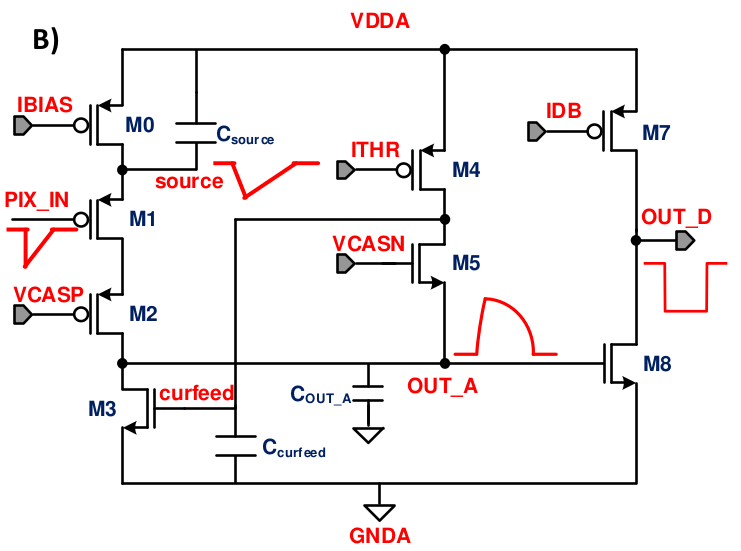
\includegraphics[width=.98\linewidth]{figures/Monopix1/ALPIDE_FE.png}
            \caption{ALPIDE-like}
            \label{fig:ALPIDE-like}
            \end{subfigure}
            \begin{subfigure}{.5\textwidth}
            \centering
            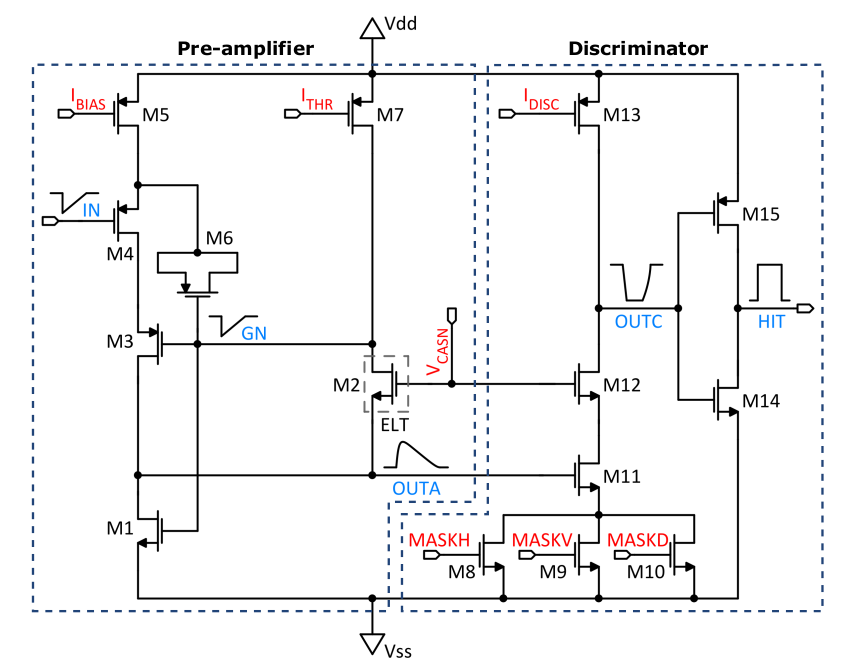
\includegraphics[width=.98\linewidth]{figures/Monopix1/Monopix1_FE_circuit.png}
            \caption{}
            \label{fig:Monopix1_FE_circuit}
            \end{subfigure}
        \end{figure}

      The idea of the amplification stage is to transfer the charge from a bigger capacity\cite{ALPIDE-FE}, $C_{source}$, to a smaller one, $C_{out}$: the input transistor M1 with current source IBIAS acts as a source follower and this forces the source of M1 to be equal to the gate input  $\Delta V_{PIX\_IN} = Q_{IN}/C_{IN}$.
      \begin{equation}
         Q_{source} = C_{source} \Delta V_{PIX\_IN}
      \end{equation}
      The current in M2 and the charge accumulates on $C_{out}$ is fixed by the one on $C_{source}$:
      \begin{equation}
         \Delta V_{OUT\_A} = \frac{Q_{source}}{C_{OUT\_A}} = \frac{C_{source}\Delta V_{PIX\_IN}}{C_{OUT\_A}}  = \frac{C_{Source}}{C_{OUT\_A}}\frac{Q_{IN}}{C_{IN}}
      \end{equation}
      A second branch (M4, M5) is used to generate a low frequency feedback, where VCASN and ITHR set the baseline value of the signal on $C_{OUT\_A}$ and the velocity to goes down to the baseline.\\
      \red{IL RUOLO DI CURVFEED NON L'HO CAPITO.}\\
      Finally IDB defines the charge threshold with which the signal $OUT\_A$ must be compared: depending on if the signal is higher than the threshold or not, the $OUT\_D$ is high or low respectively.

    The FE circuit \ref{fig:Monopix1_FE_circuit} is ALPIDE-like, so it is similar to the one described in \ref{chap:}; a quanto già detto voglio però aggiungere due parole: come viene implementato il mascheramento dei pixels e il reset.\\ 

    
    In order to reduce the hit rate and to avoid saturating the bandwidth, is uttermost important to include in the FE a way to mask noisy pixels, which typically are those with manufacturing defects.
    In the circuit in fig. \ref{fig:Monopix1_FE_circuit} transistors M8, M9 and M10 have the function of disabling registers with coordinates MASKH, MASKV and MASKD (respectivelly vertical, orizontal and diagonal) from readout: if all three transistors-signals are low, the pixel's discriminator is disabled. 
    Compared with a configurable masking register which would allow disableing pixels individually, to use a triple redundancy reduces the sensistivity to SEU\footnote{Single Event Upset, in sostanza è quando un bit ti cambia valore (da 0 a 1 o viceversa) perché una particella deposita carica nell'elettronica che fa da memoria registro/RAM/.... Questo tipo di elettronica ha bisogno di un sacco di carica prima che il bit si "flippi" (cambi valore), infatti tipicamente per avere un SEU non basta una MIP che attraversa esattemente quel pezzo di chip in cui è implementata la memoria, ma un adrone che faccia interazione nucleare producendo più carica di quanto farebbe una MIP. Questo metodo pur essendo più comodo richieda less amount of area ha però come drawback che il registro può essere soggetto a SEU problema non trascurabile in acceleratori come HL-LHC adronici} but also gives amount of intentionally masked ("ghost") pixels.
    This approach is suitable only for extremely small number N of pixel has to be masked: if two coordinate projection scheme had been implemented, the number of ghost pixels would have scale with $N^2$, if instead three coordinates are used, the N's exponential is lower than 2 (fig. \ref{fig:masking_scheme})
       \begin{figure}[h!]
        \centering
        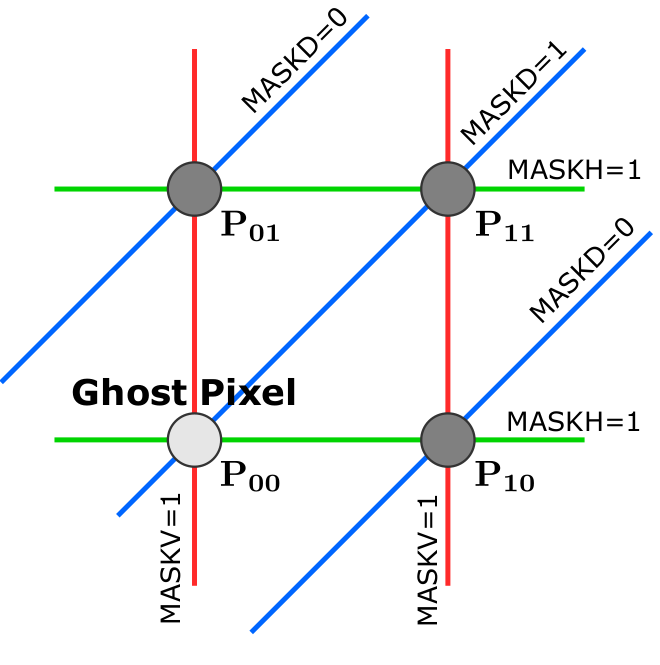
\includegraphics[width=.3\linewidth]{figures/Monopix1/masking_scheme.png}
        \caption{}
        \label{fig:masking_scheme}
    \end{figure}

    \subsection{FE parameters}
    Descrivo un po' le misure fatte sul fe e sul significato dei vari parametri.\\
    it allows injecting pixels with a known charge in DAC units. 
    \begin{table}
        \begin{center}
        \begin{tabular}{|c | c |}
        \hline
        Parameter & Meaning\\
        \hline
        \hline
        IBIAS &\\
        IDB &\\
        ITHR & \\
        VCASN &\\
        VREF &\\
        IREF &\\
        \hline
        \end{tabular}
        \caption{}
        \label{tab:FE-parameters}
        \end{center}
     \end{table}
    
\section{Readout logic}
    TJ-Monopix1 has a triggerless, fast and with ToT capability R/O which is based on a column-drain architecture.      
    On the pixel are located two Random Access Memory (RAM) cells to store the 6-bit LE and 6-bit TE of the pulse, and a Read-Only Memory (ROM) containing the 9-bit pixel address. Excluded these memories, TJ-Monopix1 hasn't any other buffer: if a hit arrives while the pixel is already storing a previous one, the new data get lost.  
    After being read, the data packet is sent to the EoC periphery of the matrix, where a serializer transfers it off-chip to an FPGA (\ref{fig:R/O-system}). There a FIFO is used to temporarily stored the data, which is transmitted to a computer through an ethernet cable in a later time.  
    \begin{figure}
        \begin{subfigure}{\textwidth}
        \centering
        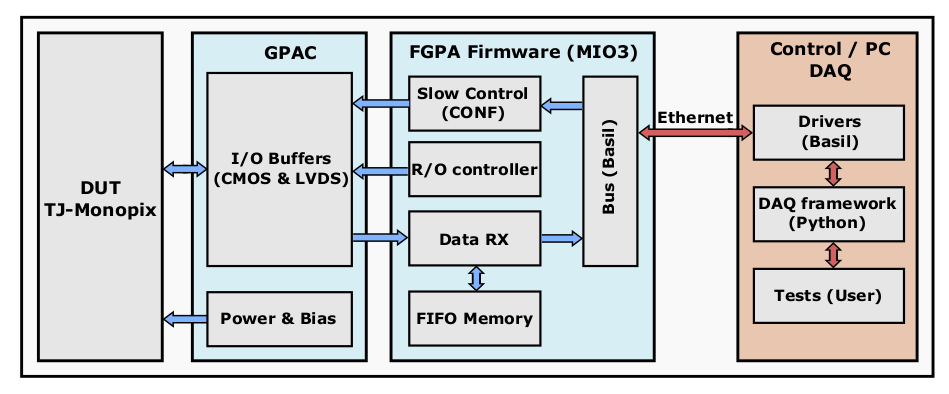
\includegraphics[clip,width=0.8\linewidth]{figures/Monopix1/schematic_boards.png}
        \end{subfigure}
        \bigskip
        \begin{subfigure}{\textwidth}
        \centering    
        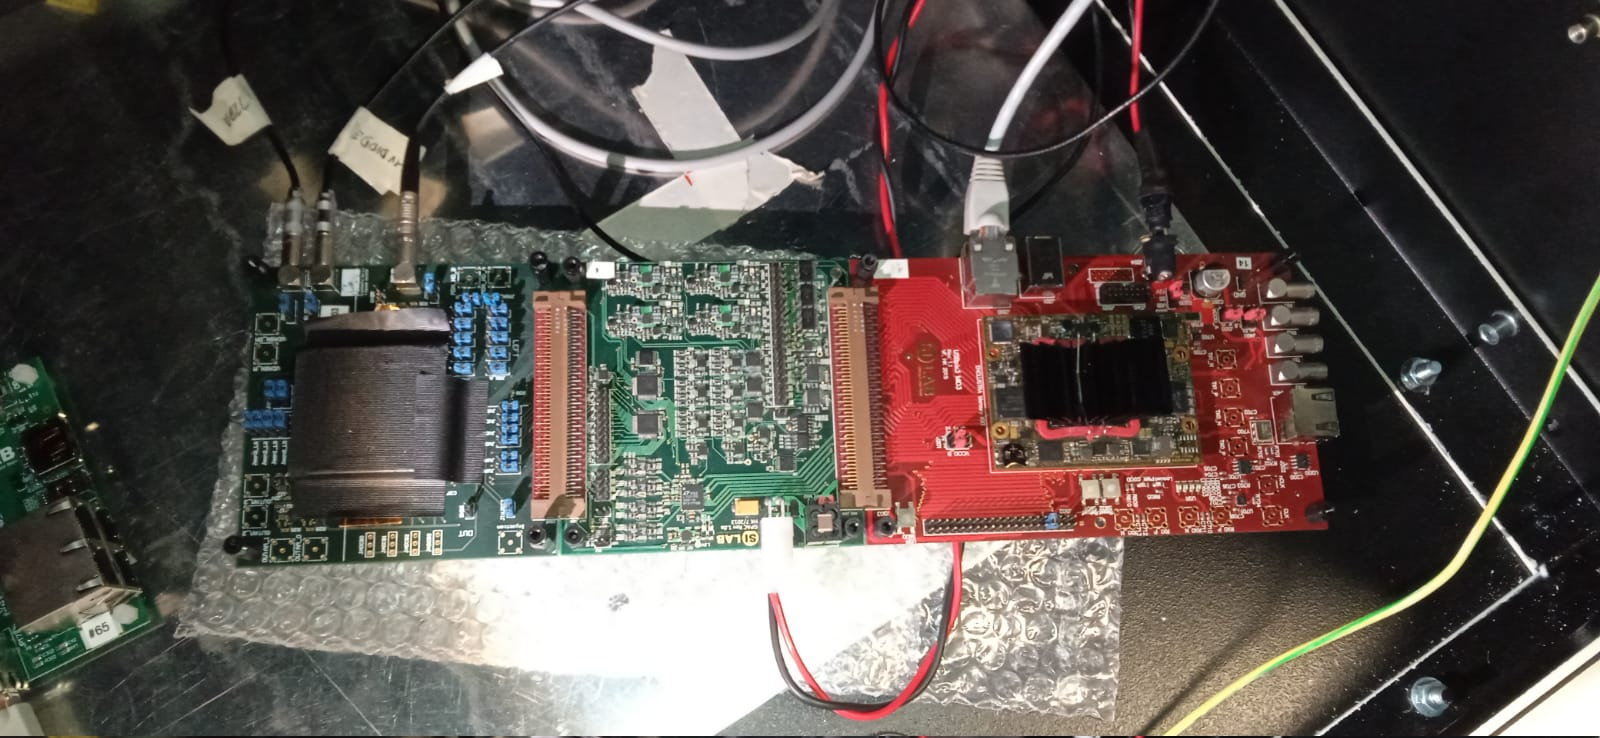
\includegraphics[clip,width=0.8\linewidth]{figures/Monopix1/monopix1_front.jpeg}
        \end{subfigure}
        \caption{Main caption}
        \label{fig:R/O-system}
    \end{figure}


    The access to the pixels' memory and the transmission of the data to the EoC is based on a Finite State Machine (FSM) composed by four state: no-operation (NOP), freeze (FRZ), read (RD) and data transfer (DTA). The readout sequence (\ref{fig:readout_schematics}) starts with the TE of a pulse: the pixel immediately tries to grab the column-bus turning up a hit flag signal called \textit{token}.   
    The token is used to control the priority chain and propagates across the column indicating what pixel that must be read. To start the readout and avoid that the arrival of new hits disrupt the priority logic, a \textit{freeze} signal is activated, and then a \textit{read} signal controls the readout and the access to memory.
    During the freeze, the state of the token for all pixels on the matrix remains settled: this does not forbid new hits on other pixels from being recorded, but forbids pixels hit from turning on the token until the freeze is ended. 
    The freeze stays on until the token covers the whole priority chain and gets the EoC: during that time new token cannot be turned on, and all hits arrived during a freeze will turn on their token at the end of the previous freeze.  
    Since the start of the token is used to assign a timestamp to the hit, the token time has a direct impact on the time resolution measurement; this could be a problem coping with high hits rate. 
    \begin{figure}[h!]
        \centering
        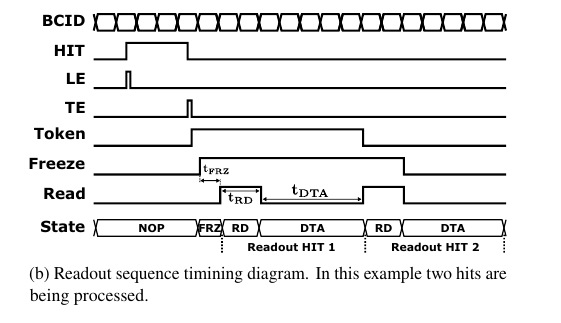
\includegraphics[width=.5\linewidth]{figures/Monopix1/readout_timing.png}
        \caption{Readout timing diagram: in this example two hits are being processed}
        \label{fig:readout_schematics}
    \end{figure}

    The analog FE circuit and the pixel control logic are connected by an edge detector which is used to determine the LE and the TE of the hit pulse(fig. \ref{fig:pixel_logic}): when the TE is stored in the first latch the edge detector is disabled and, if the \textcolor{red}{FREEZE} signal is not set yet, the readout starts. 
    At this point the HIT flag is set in a second latch and a token signal is produced and depending on the value of \textcolor{Cerulean}{Token in} the pixel can be read or must wait until the \textcolor{Cerulean}{Token in} is off. In figure an OR is used to manage the token propagation, but since a native OR logic port cannot be implemented with CMOS logic, a sum of a NOR and of an inverter is actually used; this construct significantly increases the propagation delay (the timing dispersion along a column of 0.1-0.2 ns) of the token and to speed up the circuit optimized solution are often implemented.  
    When the pixel become the next to be read in the queue, and at the rising edge of the \textcolor{red}{READ} signal, the state of the pixel is stored in a D-latch and the pixel is allowed to use the data bus; the TE and the HIT flag latches are reset and a \textcolor{Cerulean}{READINT} signal that enable access of the RAM and ROM cells is produced.\\
    \begin{figure}[h!]
        \centering
        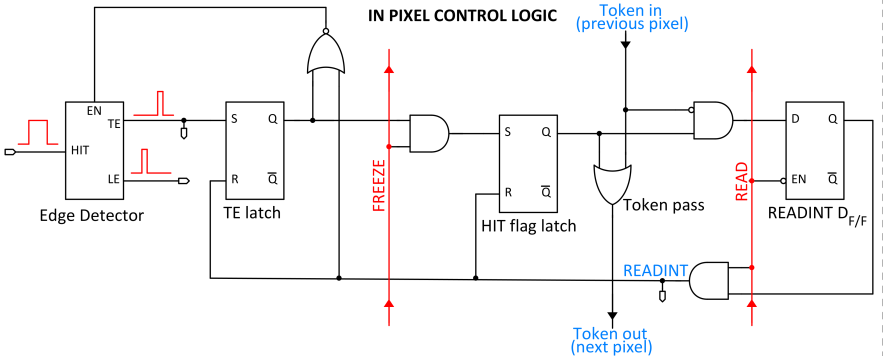
\includegraphics[width=.9\linewidth]{figures/Monopix1/Monopix1_readout_schematics.png}
        \caption{}
        \label{fig:pixel_logic}
    \end{figure}
    

    
    The final data must provide all the hits' information: the pixel address, the ToT and the timestamp. All those parts are assigned and appended at different time during the R/O chain:  
    \begin{itemize}
        \item\textbf{Pixel address:} while the double column address (6-bit) is appended by the EoC circuit, the row address (8-bits for each flavor) and the physical column in the doublet (1-bit) are assigned by the in-pixel logic      
        \item \textbf{ToT:} is obtained offline from the difference of 6-bits TE and 6-bits LE, stored by the edge detector in-pixel; since a 40 MHz BCID is distributed across the matrix, the ToT value is range 0-64 clock cycle which corresponds to 0-1.6 \si{\mu s}  
        \item \textbf{Timestamp:} The timestamp of the hit correspond to the time when the pixel set up the token; it is assigned by the FPGA, that uses the LE, TE and a 640 MHz clock to derive it
    \end{itemize}
    When the bits are joined up together the complete hit data packet is 27-bit. 

    \subsection{Dead time measurement}
        Only one hit at a time can be stored on the pixel's RAM, so until the data have completed the path to get out, the pixel readout is paralyzed; so, the dead time corresponds with the time needed to export the data-packets. 
        Since at the EoC there is one serializer per flavor, there is a linear dependence of the dead time depends 
        
        Dal momento che c'è un solo serializzatore e che quindi la lettura è sequenziale per tutto il flavor e per quanto detto sul funzionamento del R/O, il $\tau$ dipende in maniera lineare dal numero di pixel contenenti una hit. Per verificare l'andamento lineare e valurare quanto fosse il tempo morto in funzione del rate ho effettuato uno scan nel rate (diminuendo il periodo tra gli impulsi) e nel numero di pixel iniettati. 

        Il collo di bottiglia del tempo morto è dato dal fatto che c'è un unico serializzatore, infatti per trasmettere i dati dal pixel alla EoC è necessario un solo ciclo di clock dal momento che c'è un data bus da n-bit. 
        Per definre meglio il $\tau$ faccio riferimento alla fig \ref{tempidilettura}: se una hit arriva su un pixel mentre ha il token alto allora la hit viene persa. Se una hit arriva su un pixel che non ha il token alto ma ha il freeze alto, allora non viene persa ma le viene assegnato un timestamp errato. 
        To measure the dead time I've used the injection circuit available on matrix that allows fixing not only the amplitude of the pulse (charge in DAC) but also the period and width. 

        Reducing the distance between two consecutive pulses and finding the value when the efficiency decrease, one can extimates the dead time. 

        \begin{figure}[h!]
                \centering
                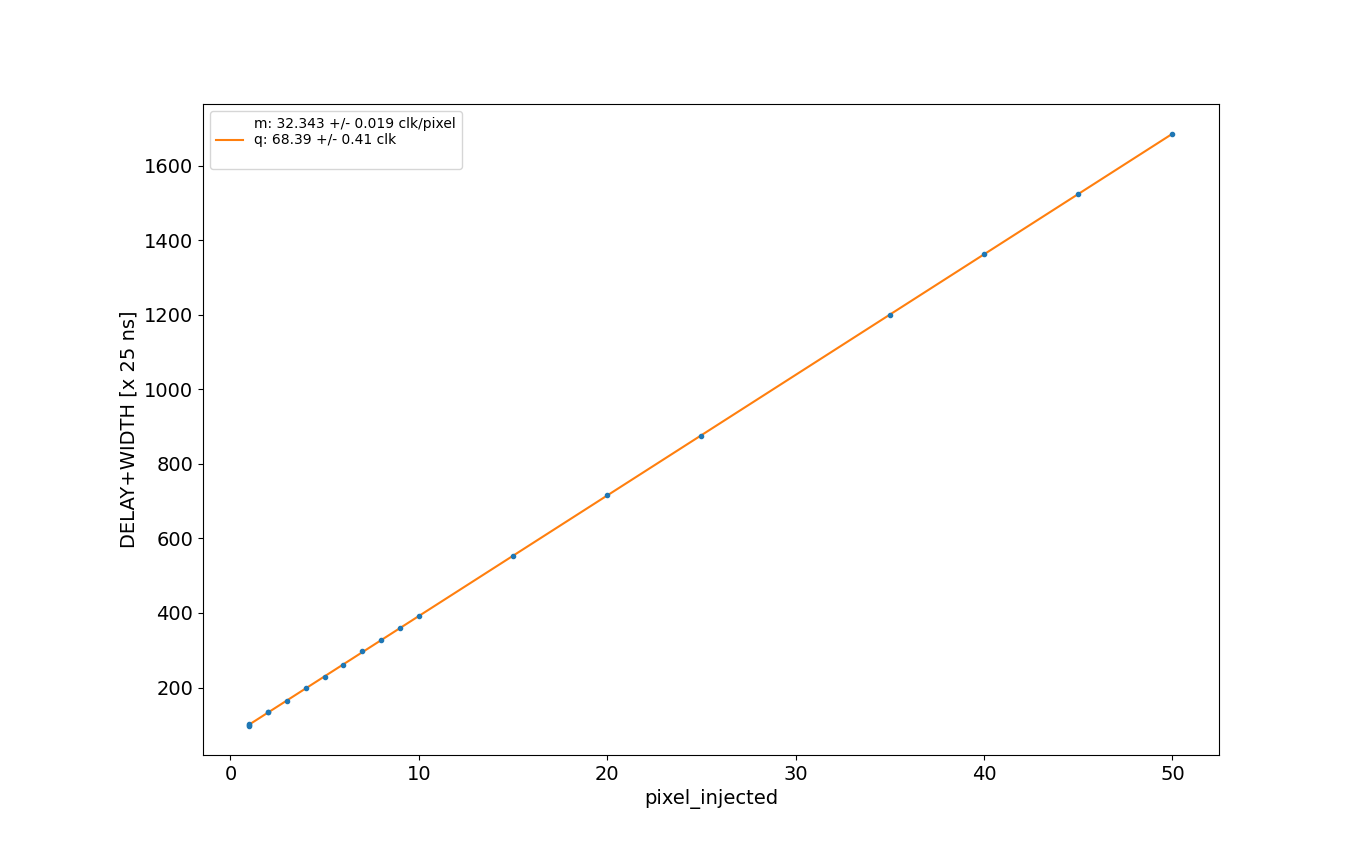
\includegraphics[width=.7\linewidth]{figures/Monopix1/dead_time.png}
                \caption{}
                \label{fig:dead_time}
            \end{figure}
        A tutte le hit di una iniezione che arrivano contemporaneamente viene assegnato lo stesso timestamp; quando le hit iniziano ad essere meno di quelle che mi aspetti.
        Mappa in funzione delle iniezioni di quali pixel hai letto.
        
    
